\documentclass[11pt]{article}
\usepackage[margin=1in]{geometry}
\usepackage{hyperref}
\usepackage{listings}
\usepackage{xcolor}
\usepackage{booktabs}
\usepackage{graphicx}

\lstset{
    basicstyle=\ttfamily\small,
    breaklines=true,
    frame=single,
    backgroundcolor=\color{gray!10}
}

\title{Cryptography and Network Security \\ Integrated Situation Technical Report}
\author{Roll No: 4202670040 \\ ULK Polytechnic Institute}
\date{\today}

\begin{document}
\maketitle

\section{Introduction}
This report covers the security review of a polytechnic institute that stores student records
on a central server and transfers files between two campuses. A prior review identified weak
staff passwords, outdated software, unencrypted file transfers, and guest network access to the
records server, along with repeated connection attempts from an unfamiliar external address.
This report presents a risk assessment of the scenario, a Python toolkit implementing file
encryption and integrity verification, and firewall rules restricting network access to the
records server, together with test evidence for each.

\section{Risk Assessment}
\subsection{Assets, Vulnerabilities and Consequences}


\begin{center}
\begin{tabular}{@{}p{3.8cm}p{4.2cm}p{5.5cm}@{}}
\toprule
Asset & Vulnerability & Consequence \\
\midrule
Central student records server & Weak staff passwords & Unauthorized access to student records, data theft or tampering \\
File transfer between campuses & Unencrypted file transfers & Interception of records in transit (eavesdropping / man-in-the-middle) \\
Records server network access & Guest network access to the records server & An unauthenticated device on the guest network could reach and attack the server \\
\bottomrule
\end{tabular}
\end{center}

\subsection{Risk Ranking}

\begin{center}
\begin{tabular}{@{}llll@{}}
\toprule
Rank & Risk & Likelihood & Impact \\
\midrule
1 & Guest network access to server & High & High \\
2 & Weak staff passwords & Medium & High \\
3 & Unencrypted file transfers & Medium & Medium \\
\bottomrule
\end{tabular}
\end{center}

Guest network access was ranked highest because the scenario reports repeated connection
attempts from an unfamiliar external address, indicating this risk is already being actively
probed rather than merely theoretical. Weak staff passwords were ranked second: likely to be
exploited given how common credential guessing is, with high impact if it succeeds. Unencrypted
transfers were ranked third, as intercepting them typically requires the attacker to already
have network position, a precondition partly addressed by mitigating risk 1.

\subsection{Recommended Controls}

\begin{center}
\begin{tabular}{@{}p{5.5cm}p{7.5cm}@{}}
\toprule
Risk & Recommended Control \\
\midrule
Guest network access to records server & Network segmentation — place the records server on a subnet not reachable from the guest network, enforced by firewall rules (implemented in Section 4 of this report) \\
Weak staff passwords & Enforce a password policy (minimum length/complexity) and multi-factor authentication \\
Unencrypted file transfers & Use an encrypted transfer protocol (e.g. SFTP or TLS) instead of plain FTP \\
\bottomrule
\end{tabular}
\end{center}

\section{Encryption, Decryption and Integrity Verification}
\subsection{Design}
The toolkit (\texttt{crypto\_toolkit.py}) uses symmetric encryption (Fernet, built on AES) to
encrypt and decrypt the sample student record file, and SHA-256 to compute an integrity
hash that can later detect whether the file has been modified.

\subsection{Execution and Evidence}

The toolkit was run on Windows PowerShell against a sample student record file. Full terminal
output is captured in Figure~\ref{fig:crypto-run}.

\begin{lstlisting}
PS> python crypto_toolkit.py generate-key secret.key
Key generated and saved to secret.key

PS> python crypto_toolkit.py encrypt sample_student_record.txt sample_student_record.enc secret.key
Encrypted 'sample_student_record.txt' -> 'sample_student_record.enc'

PS> python crypto_toolkit.py decrypt sample_student_record.enc sample_student_record.dec secret.key
Decrypted 'sample_student_record.enc' -> 'sample_student_record.dec'

PS> fc.exe sample_student_record.txt sample_student_record.dec
Comparing files sample_student_record.txt and SAMPLE_STUDENT_RECORD.DEC
FC: no differences encountered

PS> python crypto_toolkit.py hash sample_student_record.txt
SHA-256 of 'sample_student_record.txt': a2c6ec5cad425e11fbc69431d0235d5243e118bd0db7f84e57930cdf518aa336
Saved to 'sample_student_record.txt.sha256'

PS> python crypto_toolkit.py verify sample_student_record.txt sample_student_record.txt.sha256
Integrity check PASSED: file has not changed.

PS> python crypto_toolkit.py encrypt does_not_exist.txt out.enc secret.key
Error: Input file not found: does_not_exist.txt
\end{lstlisting}

\texttt{fc.exe} confirmed the decrypted file is byte-for-byte identical to the original,
the SHA-256 verification passed on the unmodified file, and attempting to encrypt a
non-existent file produced a clean error message rather than a crash, satisfying task 2d.

\begin{figure}[h]
  \centering
  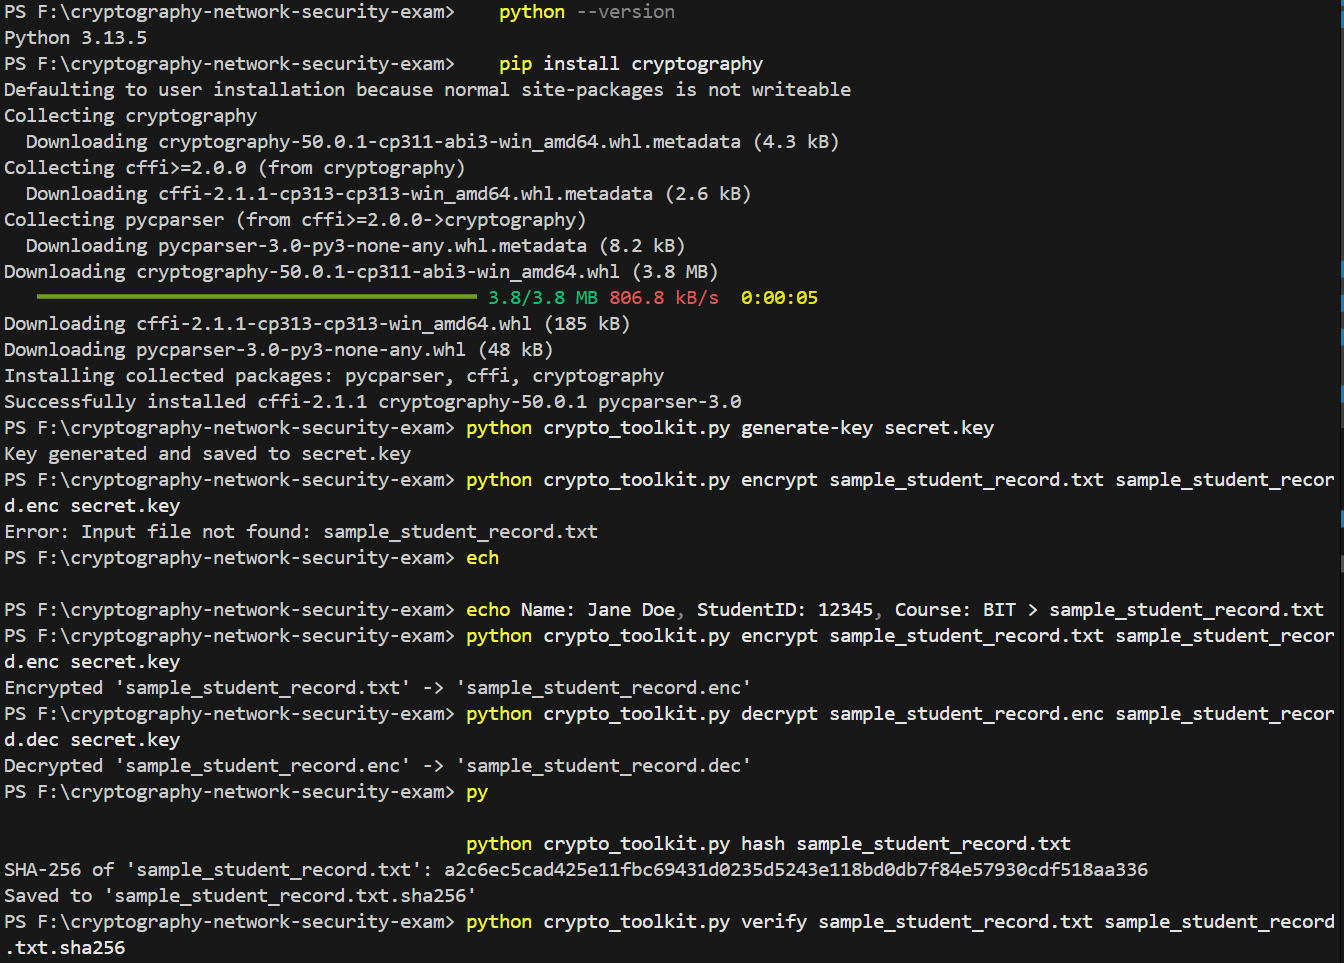
\includegraphics[width=0.9\textwidth]{evidence/crypto_toolkit_run.png}
  \caption{Terminal output of the encryption, decryption and hashing workflow.}
  \label{fig:crypto-run}
\end{figure}

\section{Network Traffic Filtering}
\subsection{Environment}
Testing was carried out on a Windows 11 laptop using Windows Defender Firewall (via the
\texttt{NetFirewallRule} PowerShell cmdlets) in place of \texttt{iptables}/\texttt{ufw}, since no
dedicated Linux lab machine was available. A Python HTTP server on port 5000 simulated the
student records service. The laptop hosted its own Mobile Hotspot so a phone could connect as
a genuinely separate device, avoiding the client-isolation restriction present on the original
mobile hotspot network.

\subsection{Firewall Rules Applied}
\begin{lstlisting}
$staffIP = "192.168.137.24"
New-NetFirewallRule -DisplayName "Block-Others-5000" -Direction Inbound -Protocol TCP `
    -LocalPort 5000 -RemoteAddress Any -Action Block
New-NetFirewallRule -DisplayName "Allow-Staff-5000" -Direction Inbound -Protocol TCP `
    -LocalPort 5000 -RemoteAddress $staffIP -Action Allow
\end{lstlisting}

\noindent\textbf{Note:} Windows Defender Firewall gives Block rules unconditional precedence
over Allow rules, unlike \texttt{iptables} where rule order determines precedence. The two
rules were therefore toggled with \texttt{Enable}/\texttt{Disable-NetFirewallRule} between
tests to produce three unambiguous results.

\subsection{Test Procedure and Results}

\textbf{Test 1 — Permitted connection.} With \texttt{Allow-Staff-5000} active and
\texttt{Block-Others-5000} disabled, the staff device (phone) loaded
\texttt{http://192.168.137.1:5000} successfully, showing a directory listing of the service
(Figure~\ref{fig:test1}).

\textbf{Test 2 — Blocked connection.} With \texttt{Block-Others-5000} enabled and
\texttt{Allow-Staff-5000} disabled, the same device could no longer reach the service; the
browser returned \texttt{ERR\_CONNECTION\_TIMED\_OUT} (Figure~\ref{fig:test2}).

\textbf{Test 3 — Blocked connection (repeat).} Under the same blocked state as Test 2, a
repeat attempt confirmed the block was consistent.

\begin{figure}[h]
  \centering
  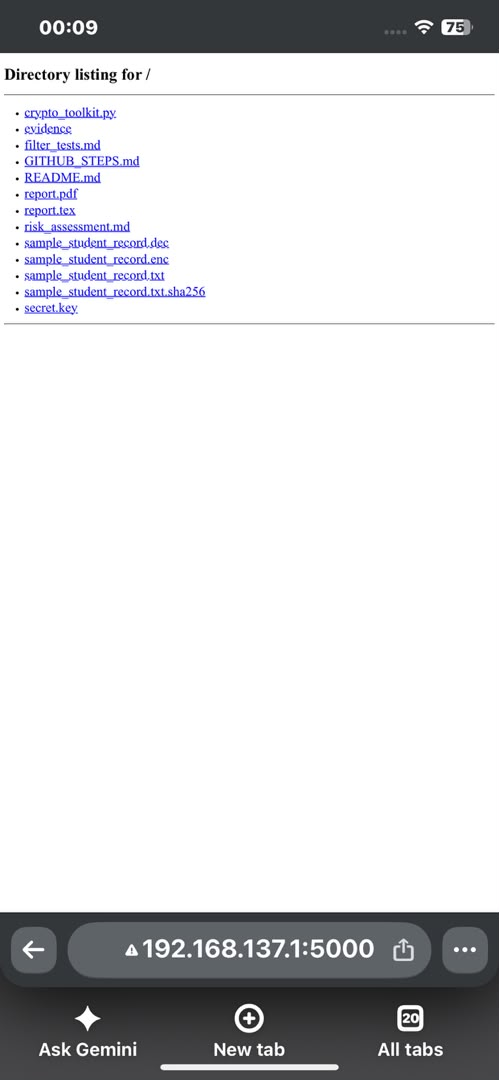
\includegraphics[width=0.6\textwidth]{evidence/test1_permitted.png}
  \caption{Test 1: permitted connection — service reachable from the staff device.}
  \label{fig:test1}
\end{figure}

\begin{figure}[h]
  \centering
  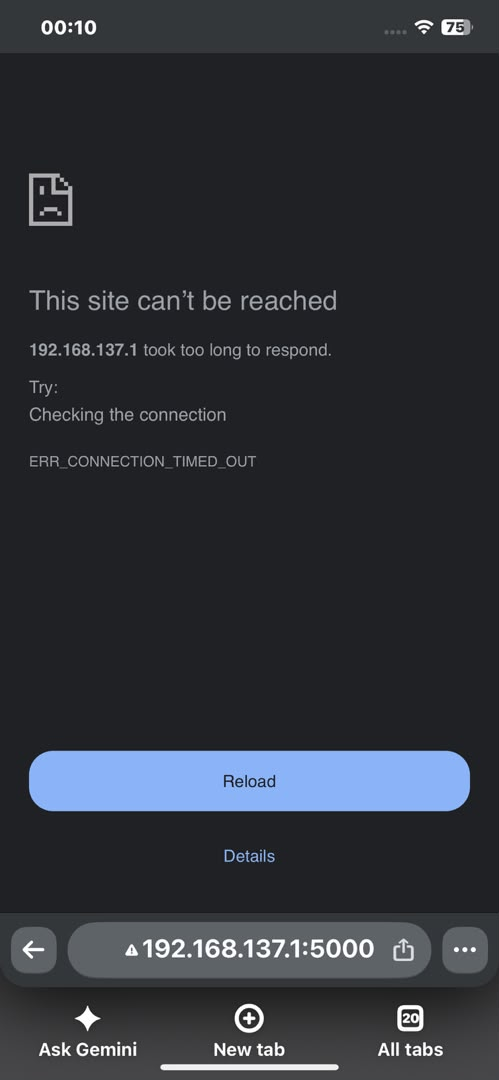
\includegraphics[width=0.6\textwidth]{evidence/test2_blocked.png}
  \caption{Test 2: blocked connection — connection timed out after the allow rule was removed.}
  \label{fig:test2}
\end{figure}

\noindent\textbf{Limitation:} only one spare physical device was available for testing rather
than three separate network segments. Tests 2 and 3 both use the same device with its
permission revoked, which still validly demonstrates that the block rule consistently denies
unauthorised access.

\section{Conclusion}
The three highest-priority risks identified were guest network access to the records server,
weak staff passwords, and unencrypted file transfers between campuses, with guest network
access ranked most urgent due to evidence of active probing already occurring. Two of the
identified risks were directly mitigated in this exercise: the encryption and integrity toolkit
addresses confidentiality and tamper-detection for stored/transferred records, while the
firewall rules address unauthorised network access by restricting the records service to a
single authorised device and blocking all other sources. Together, these controls close the two
most immediately exploitable weaknesses in the scenario. Remaining risks, particularly weak
staff passwords and outdated software, would need to be addressed through policy and patch
management measures outside the scope of the toolkit built here.

\vspace{1em}
\noindent\textbf{GitHub Repository:} \url{https://github.com/ogonjo01/cryptography-network-security-exam.git}

\end{document}
